%
% adjazenz.tex
%
% (c) 2019 Prof Dr Andreas Müller, Hochschule Rapperswil
%
\bgroup
\definecolor{darkred}{rgb}{0.5,0,0}
\begin{frame}[fragile]
\newboolean{pfeilspitzen}
\setboolean{pfeilspitzen}{true}
\frametitle{Adjazenz-Matrix}

\begin{columns}[t]
\begin{column}{0.48\hsize}
\begin{center}
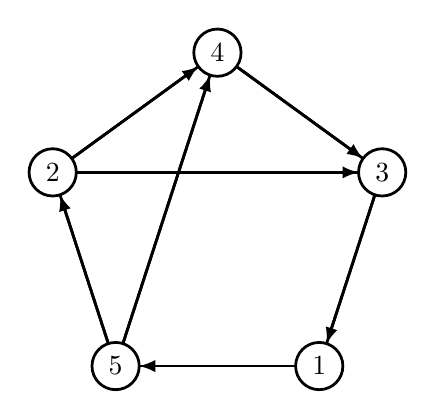
\begin{tikzpicture}[>=latex]

\def\r{2.2}
\coordinate (A) at ({\r*cos(-54+0*72)},{\r*sin(-54+0*72)});
\coordinate (C) at ({\r*cos(-54+1*72)},{\r*sin(-54+1*72)});
\coordinate (D) at ({\r*cos(-54+2*72)},{\r*sin(-54+2*72)});
\coordinate (B) at ({\r*cos(-54+3*72)},{\r*sin(-54+3*72)});
\coordinate (E) at ({\r*cos(-54+4*72)},{\r*sin(-54+4*72)});

\def\knoten#1#2{
        \fill[color=white] #1 circle[radius=0.3];
        \draw[line width=1pt] #1 circle[radius=0.3];
        \node at #1 {$#2$};
}

\def\kante#1#2#3{
        \ifthenelse{\boolean{pfeilspitzen}}{
                \draw[->,line width=1pt,shorten >= 0.3cm,shorten <= 0.3cm]
                        #1 -- #2;
        }{
                \draw[line width=1pt,shorten >= 0.3cm,shorten <= 0.3cm]
                        #1 -- #2;
        }
%        \fill[color=white,opacity=0.7] ($0.5*#1+0.5*#2$) circle[radius=0.22];
%        \node at ($0.5*#1+0.5*#2$) {$#3$};
}

\kante{(A)}{(E)}{1}
\kante{(B)}{(C)}{2}
\kante{(B)}{(D)}{13}
\kante{(C)}{(A)}{3}
\kante{(D)}{(C)}{6}
\kante{(E)}{(B)}{5}
\kante{(E)}{(D)}{6}

\knoten{(A)}{1}
\knoten{(B)}{2}
\knoten{(C)}{3}
\knoten{(D)}{4}
\knoten{(E)}{5}

\end{tikzpicture}
\end{center}
\end{column}
\begin{column}{0.48\hsize}
\[
a_{{\color{darkred}i}{\color{blue}j}}
=
\begin{cases}
1&\quad\text{\# Kanten von ${\color{blue}j}$ nach ${\color{darkred}i}$}\\
0&\quad\text{sonst}
\end{cases}
\]
\begin{center}
\begin{tikzpicture}[>=latex]
\node at (0,0) {$\displaystyle
A=
\begin{pmatrix}
0&0&1&0&0\\
0&0&0&0&1\\
0&1&0&1&0\\
0&1&0&0&1\\
1&0&0&0&0
\end{pmatrix}
$};
\def\s{0.54}
\foreach \x in {1,...,5}{
	\node[color=blue] at ({-0.71+(\x-1)*\s},1.4) {\tiny $\x$};
}
\node[color=blue] at ({-0.71+2*\s},1.7) {von};
\def\r{0.48}
\foreach \y in {1,...,5}{
	\node[color=darkred] at ({-0.71+5*\s},{0.02+(3-\y)*\r}) {\tiny $\y$};
}
\node[color=darkred] at ({-0.4+5*\s},{0.02}) [rotate=90] {nach};
\end{tikzpicture}
\end{center}
\end{column}
\end{columns}

\end{frame}
\egroup
